\subsection{Bubble chambers}
\begin{figure}

  \centering
  \begin{subfigure}[t]{0.25\textwidth}
    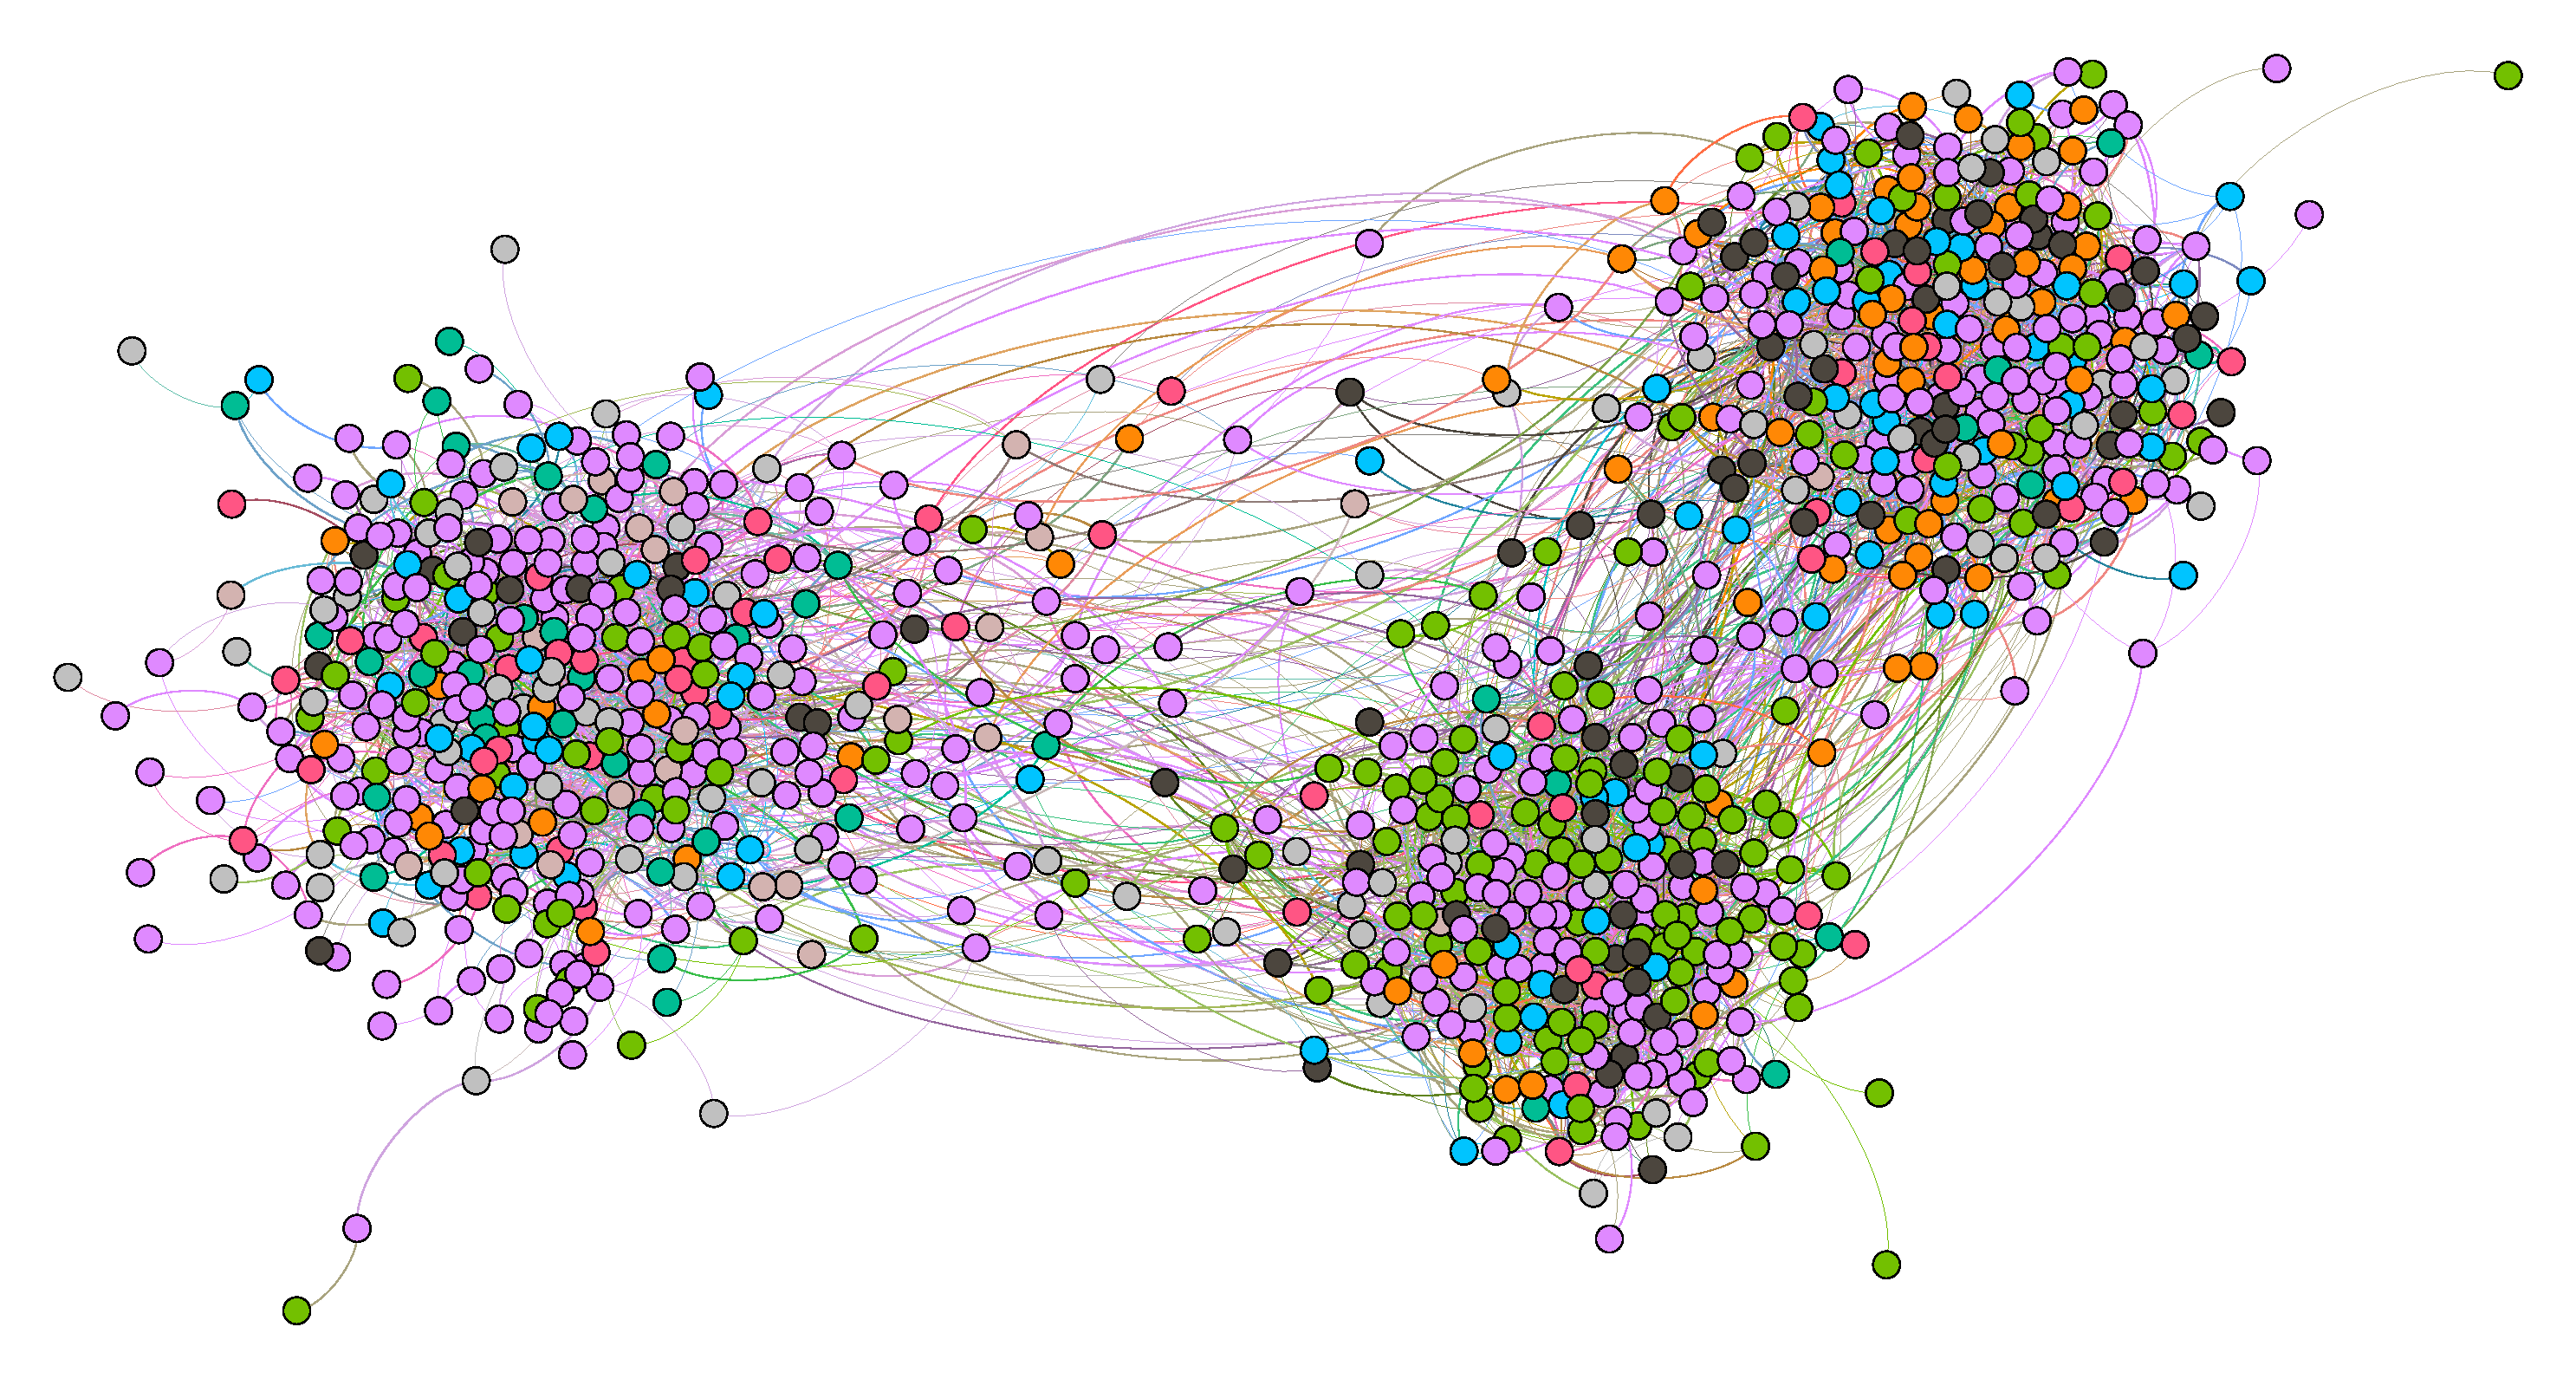
\includegraphics[width=\textwidth]{img/dim3_mod.pdf}
    \label{fig:bubble3mod}
    \caption{}
  \end{subfigure}
  ~
  \begin{subfigure}[t]{0.35\textwidth}
    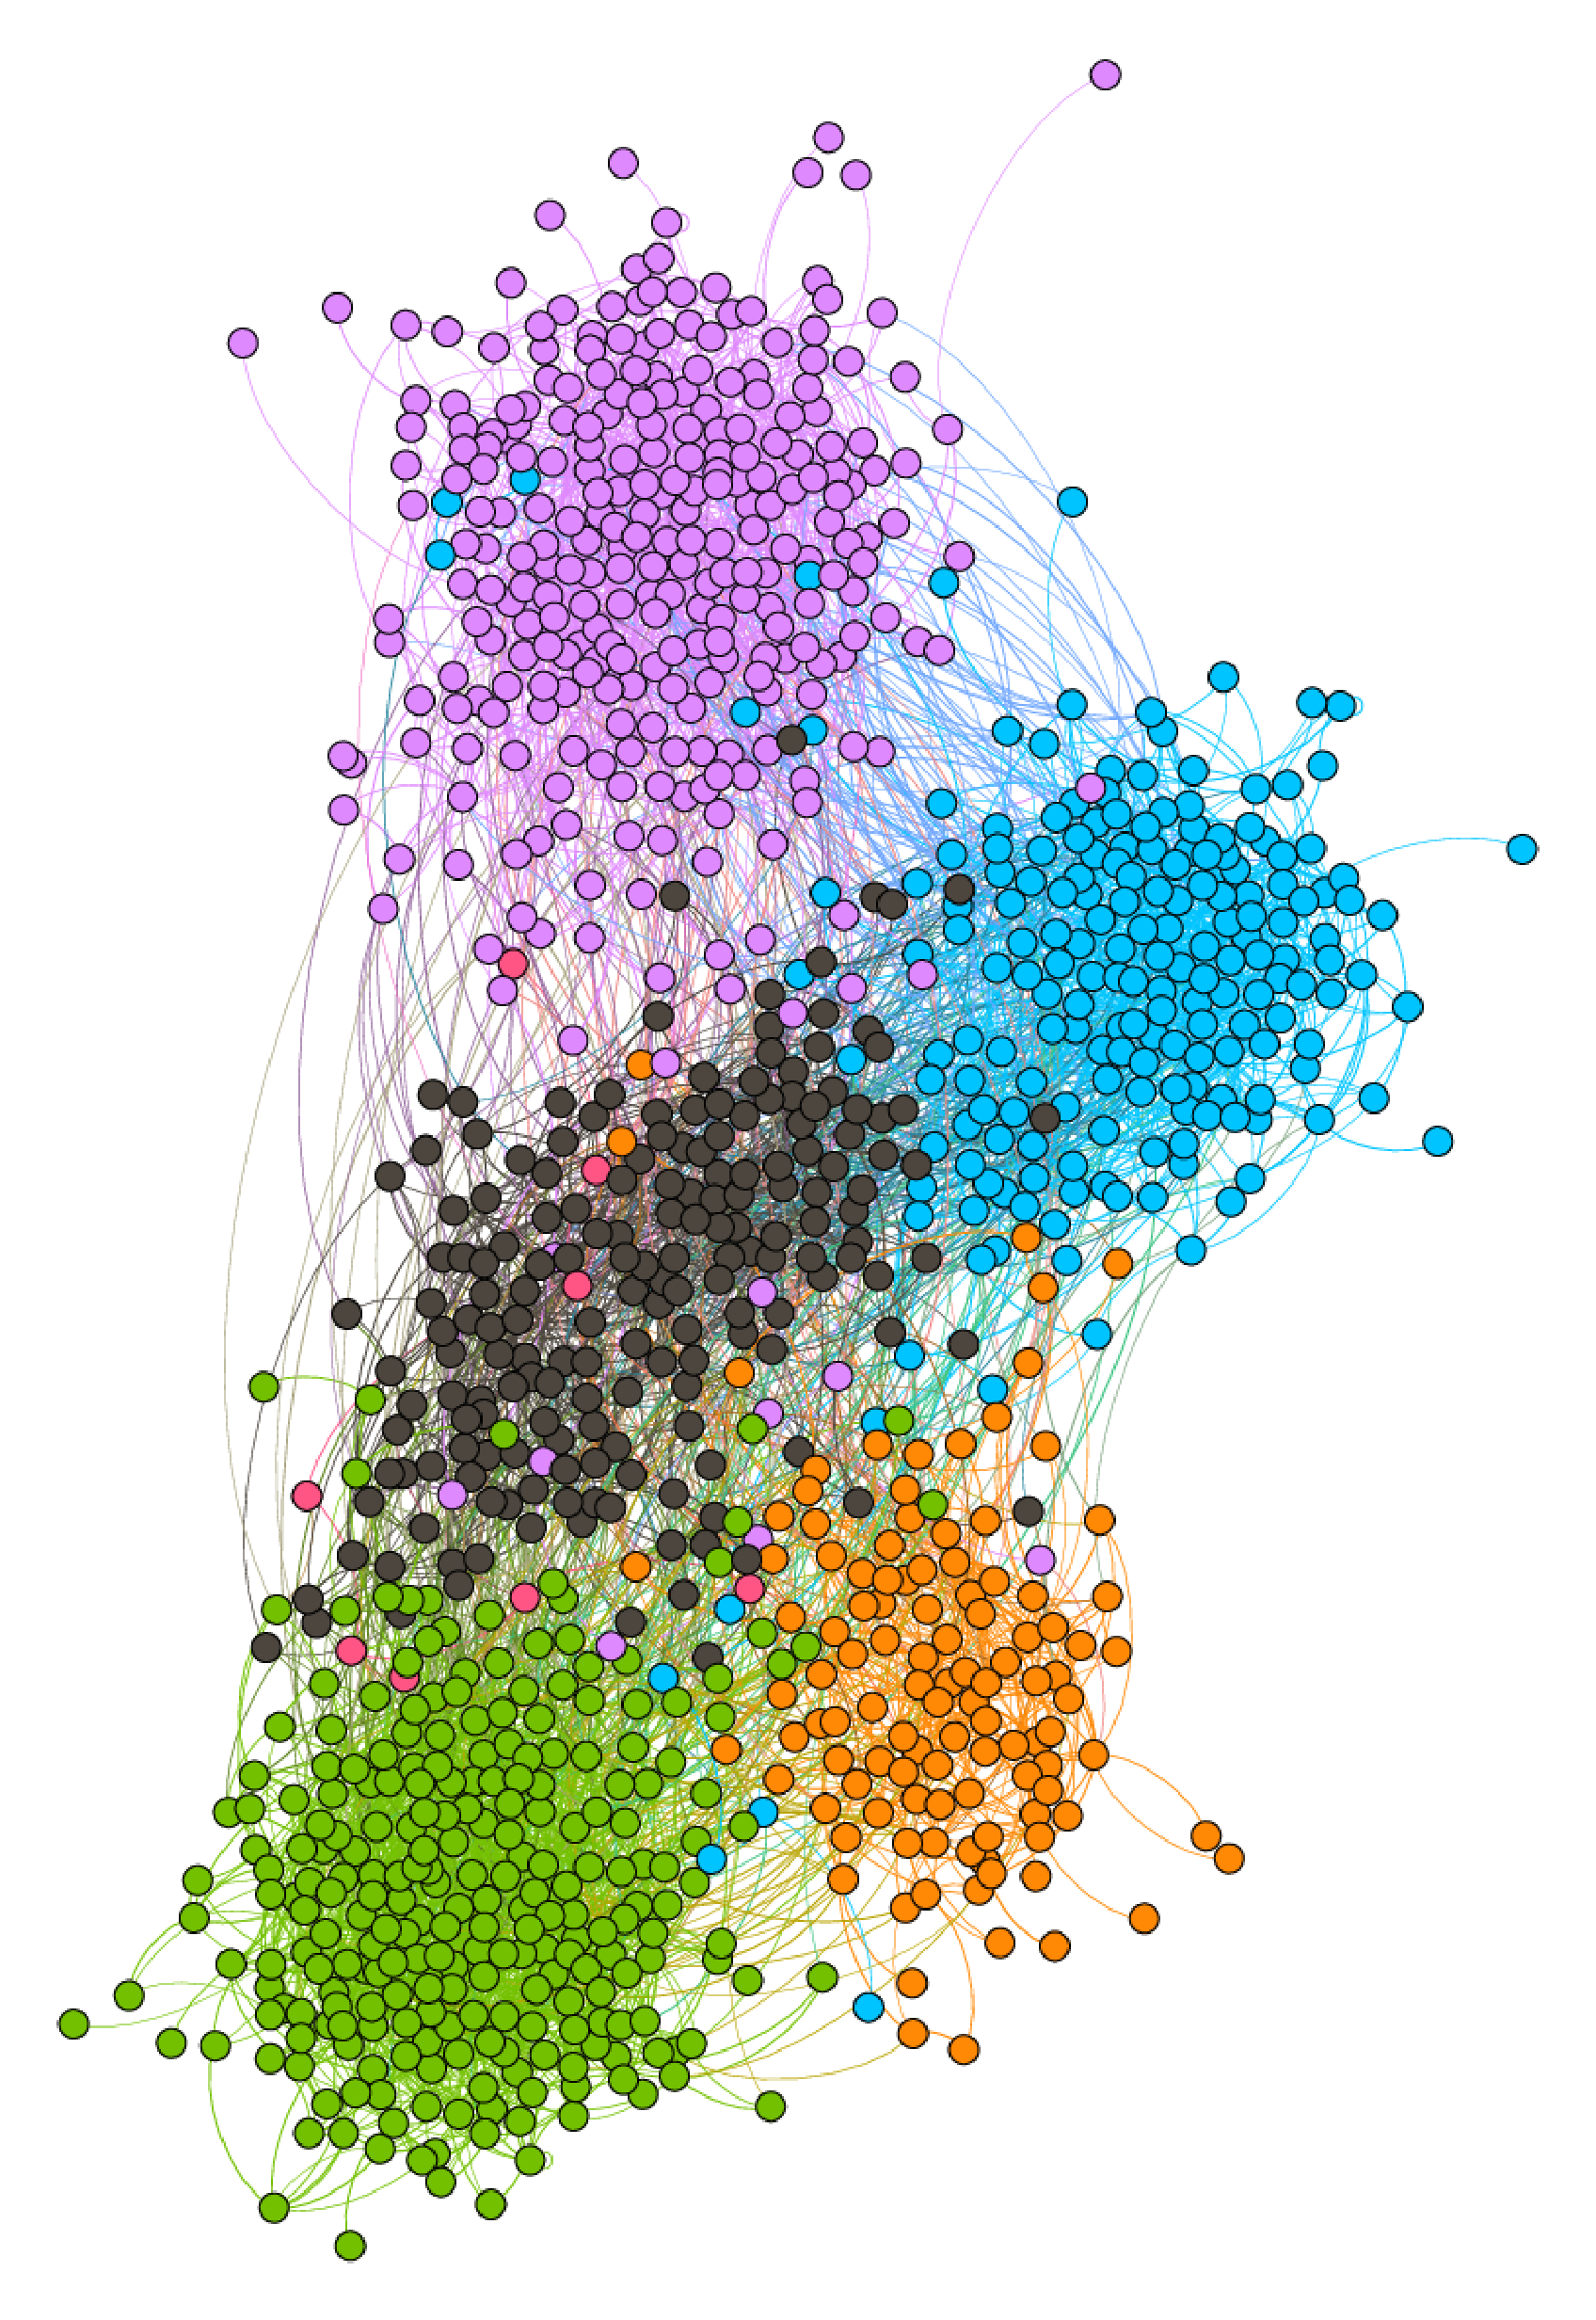
\includegraphics[width=\textwidth]{img/dim5_mod.pdf}
    \label{fig:bubble5mod}
    \caption{bubble3news}
  \end{subfigure}
  ~
  \begin{subfigure}[t]{0.35\textwidth}
    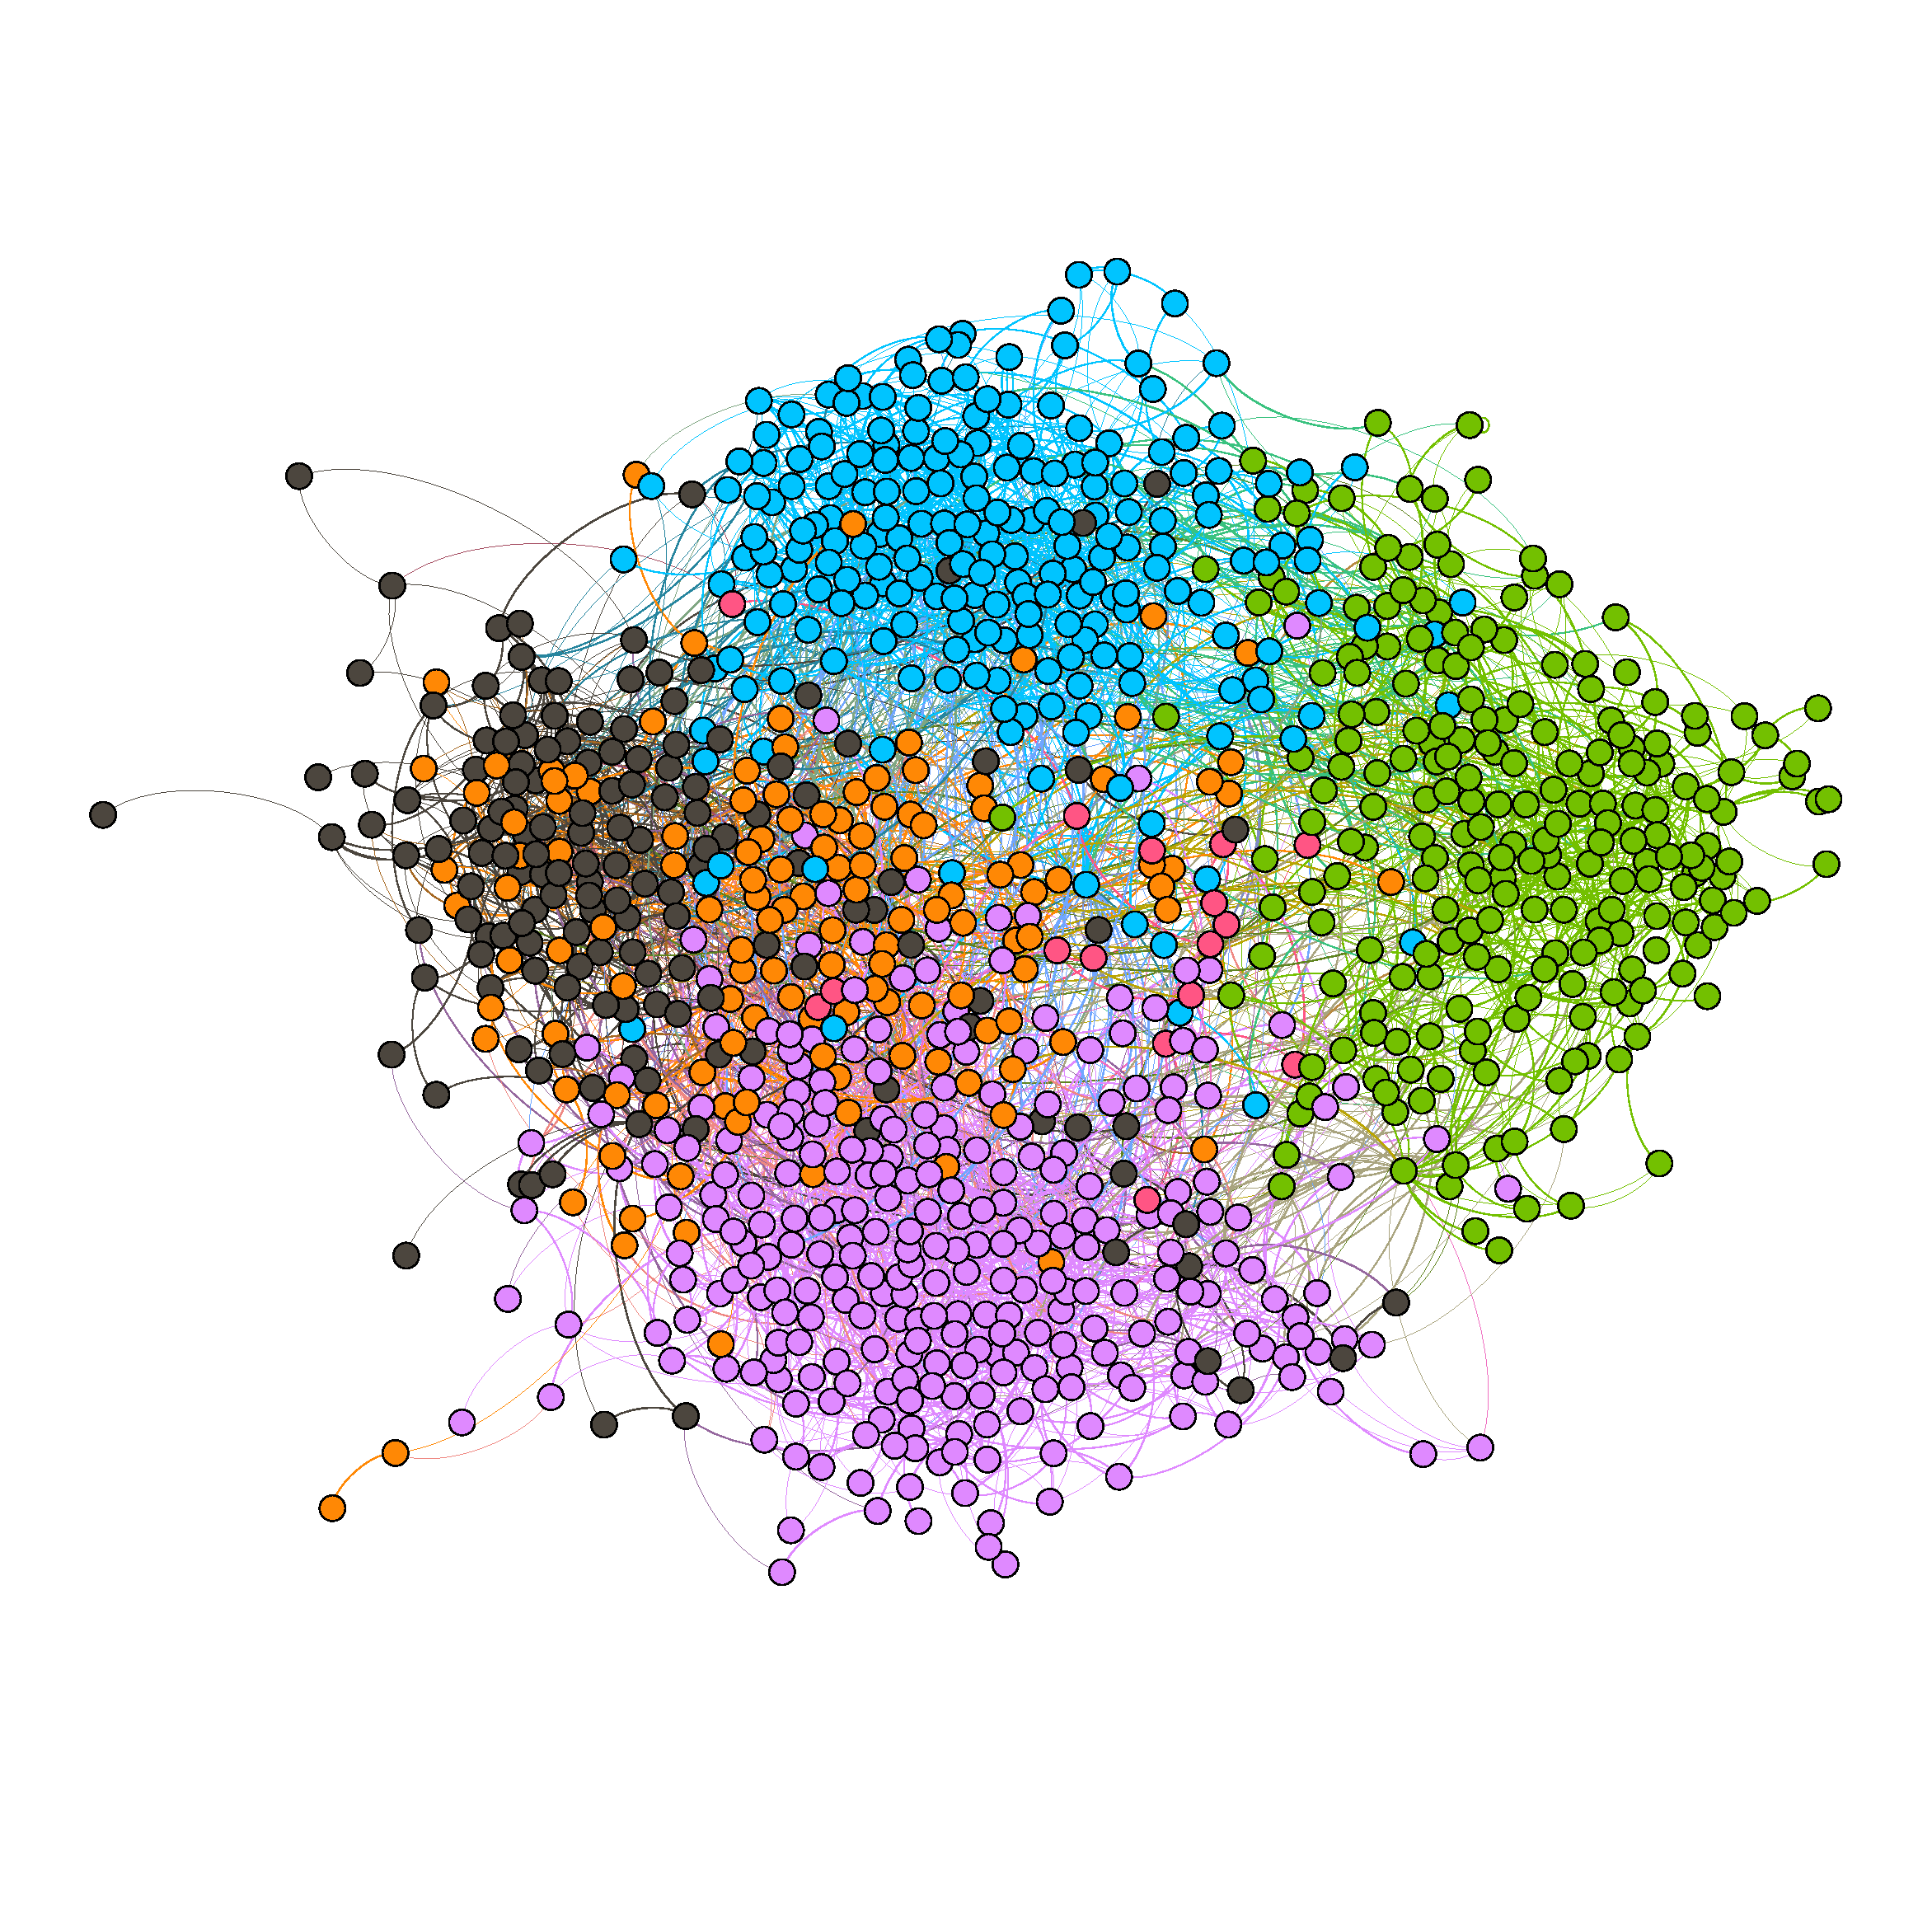
\includegraphics[width=\textwidth]{img/dim7_mod.pdf}
    \label{fig:bubble7mod}
    \caption{bubble3news}
  \end{subfigure}
  \\
  \begin{subfigure}[t]{0.25\textwidth}
    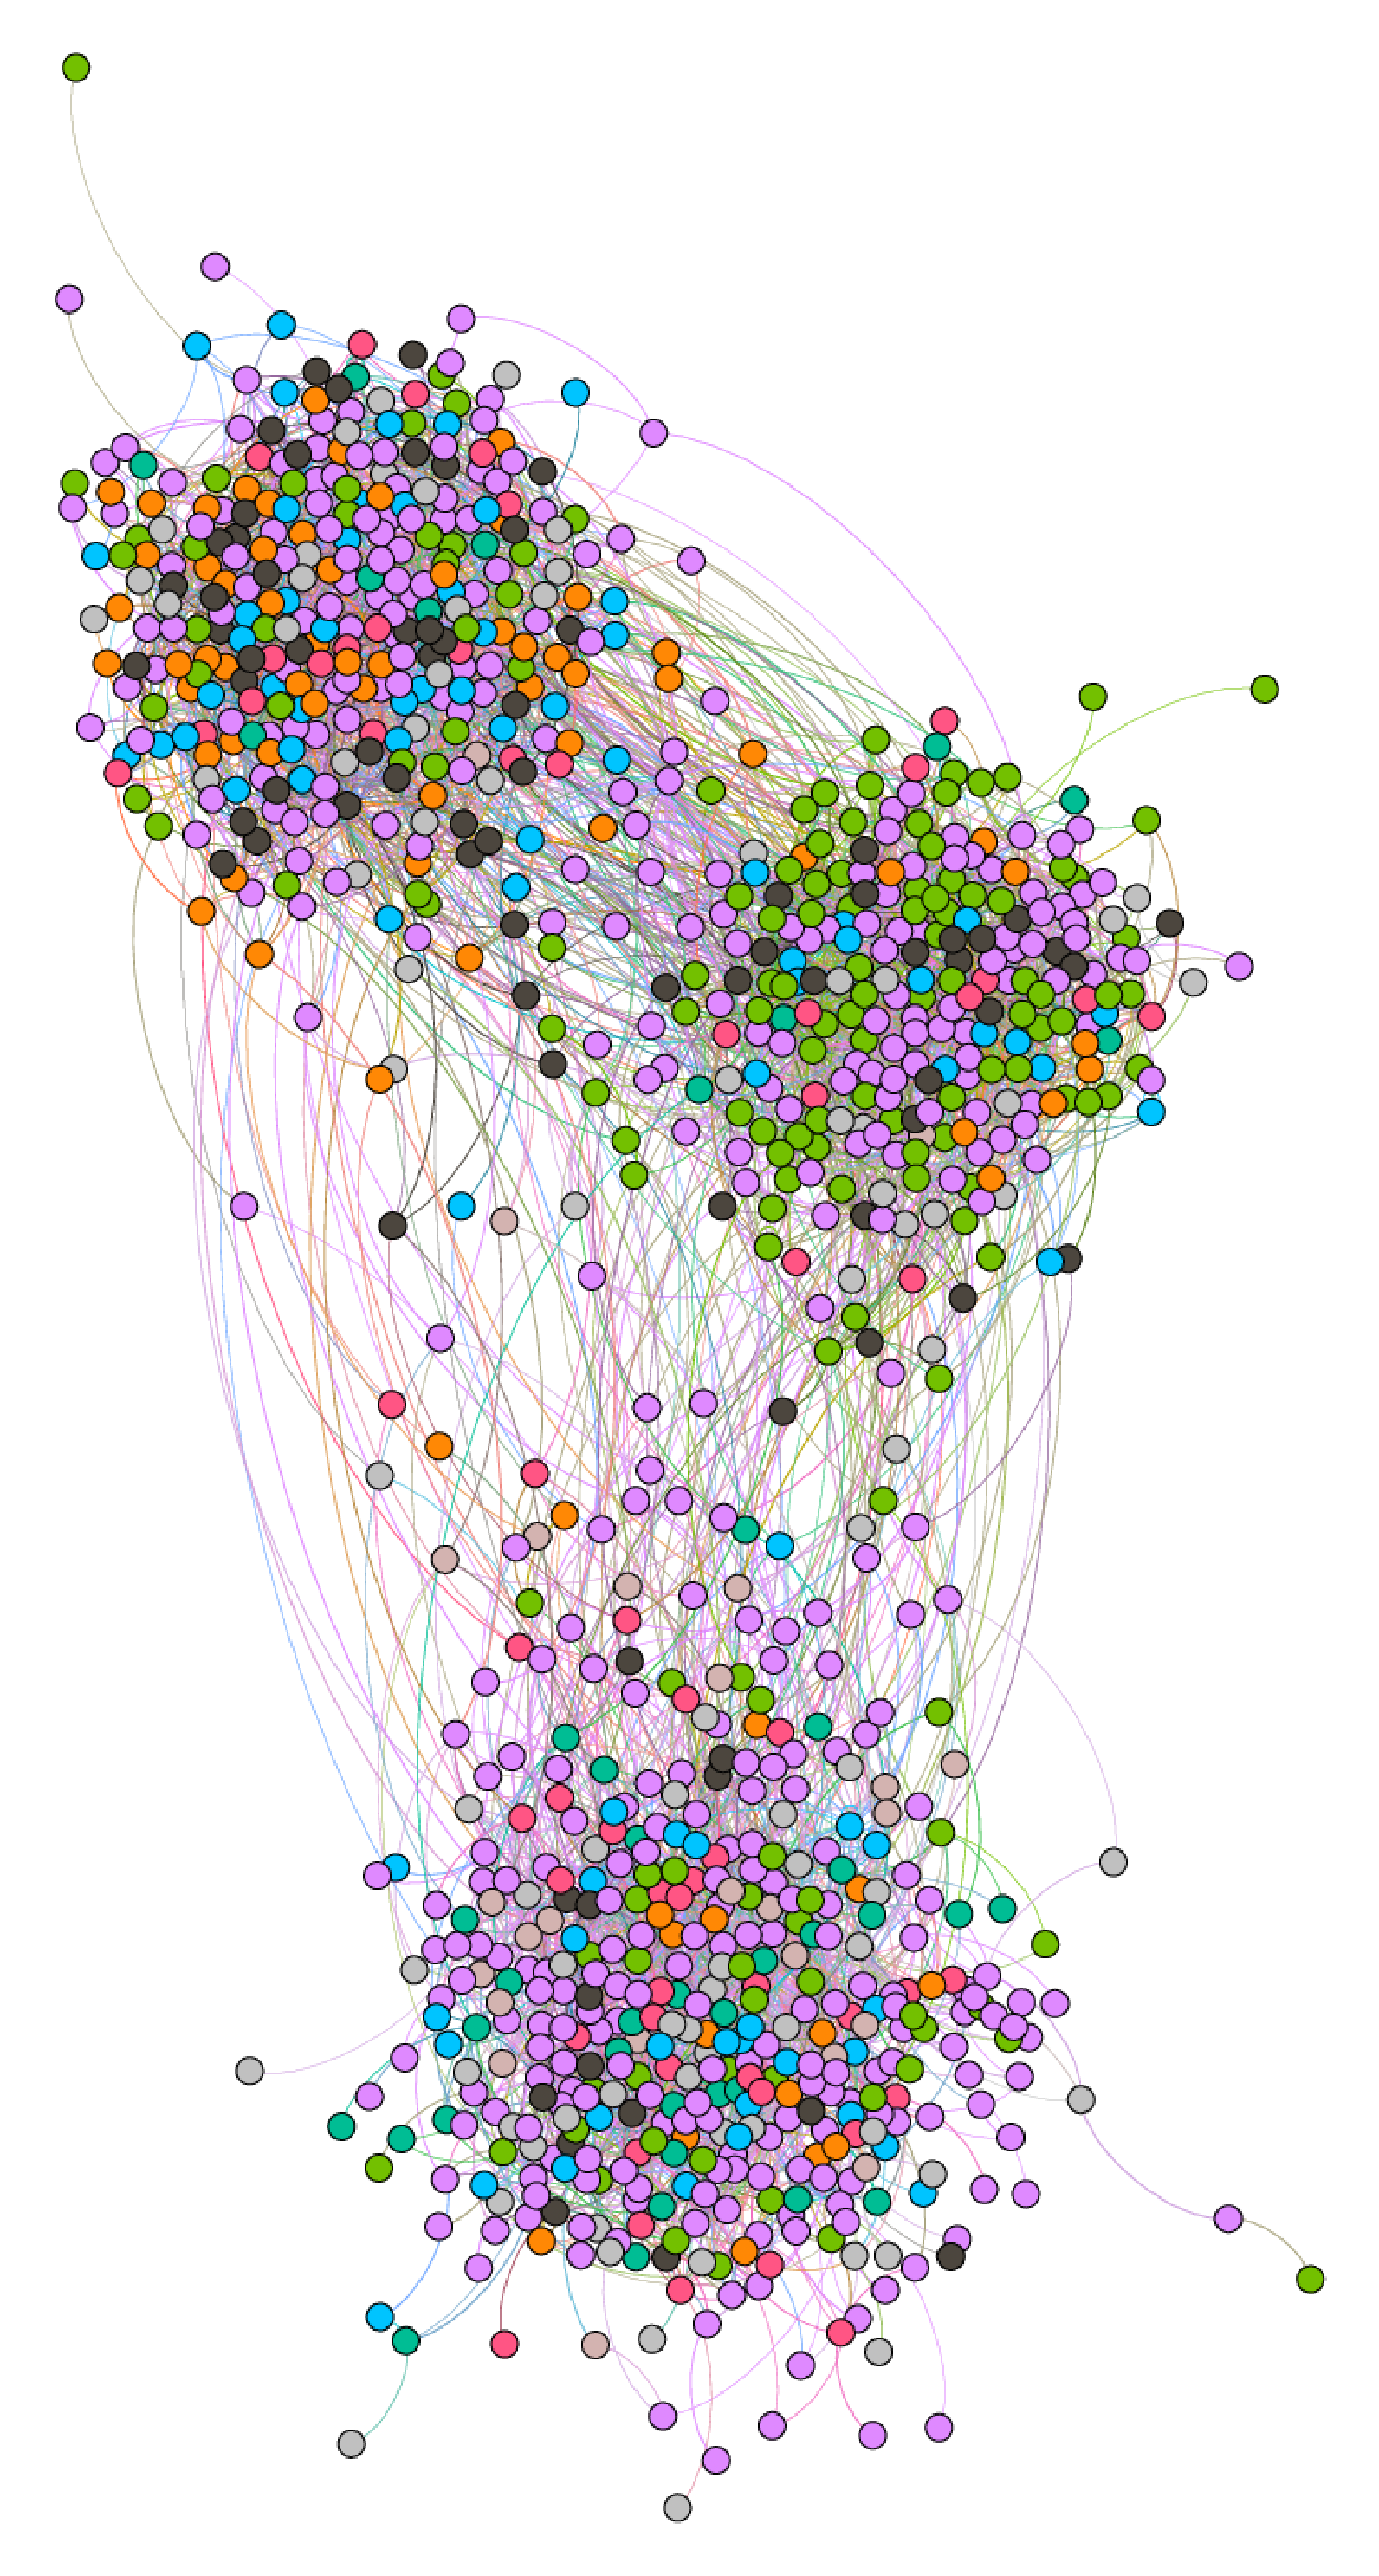
\includegraphics[width=\textwidth]{img/dim3_news.pdf}
    \label{fig:bubble3news}
    \caption{bubble3mod}
  \end{subfigure}
  ~
  \begin{subfigure}[t]{0.35\textwidth}
    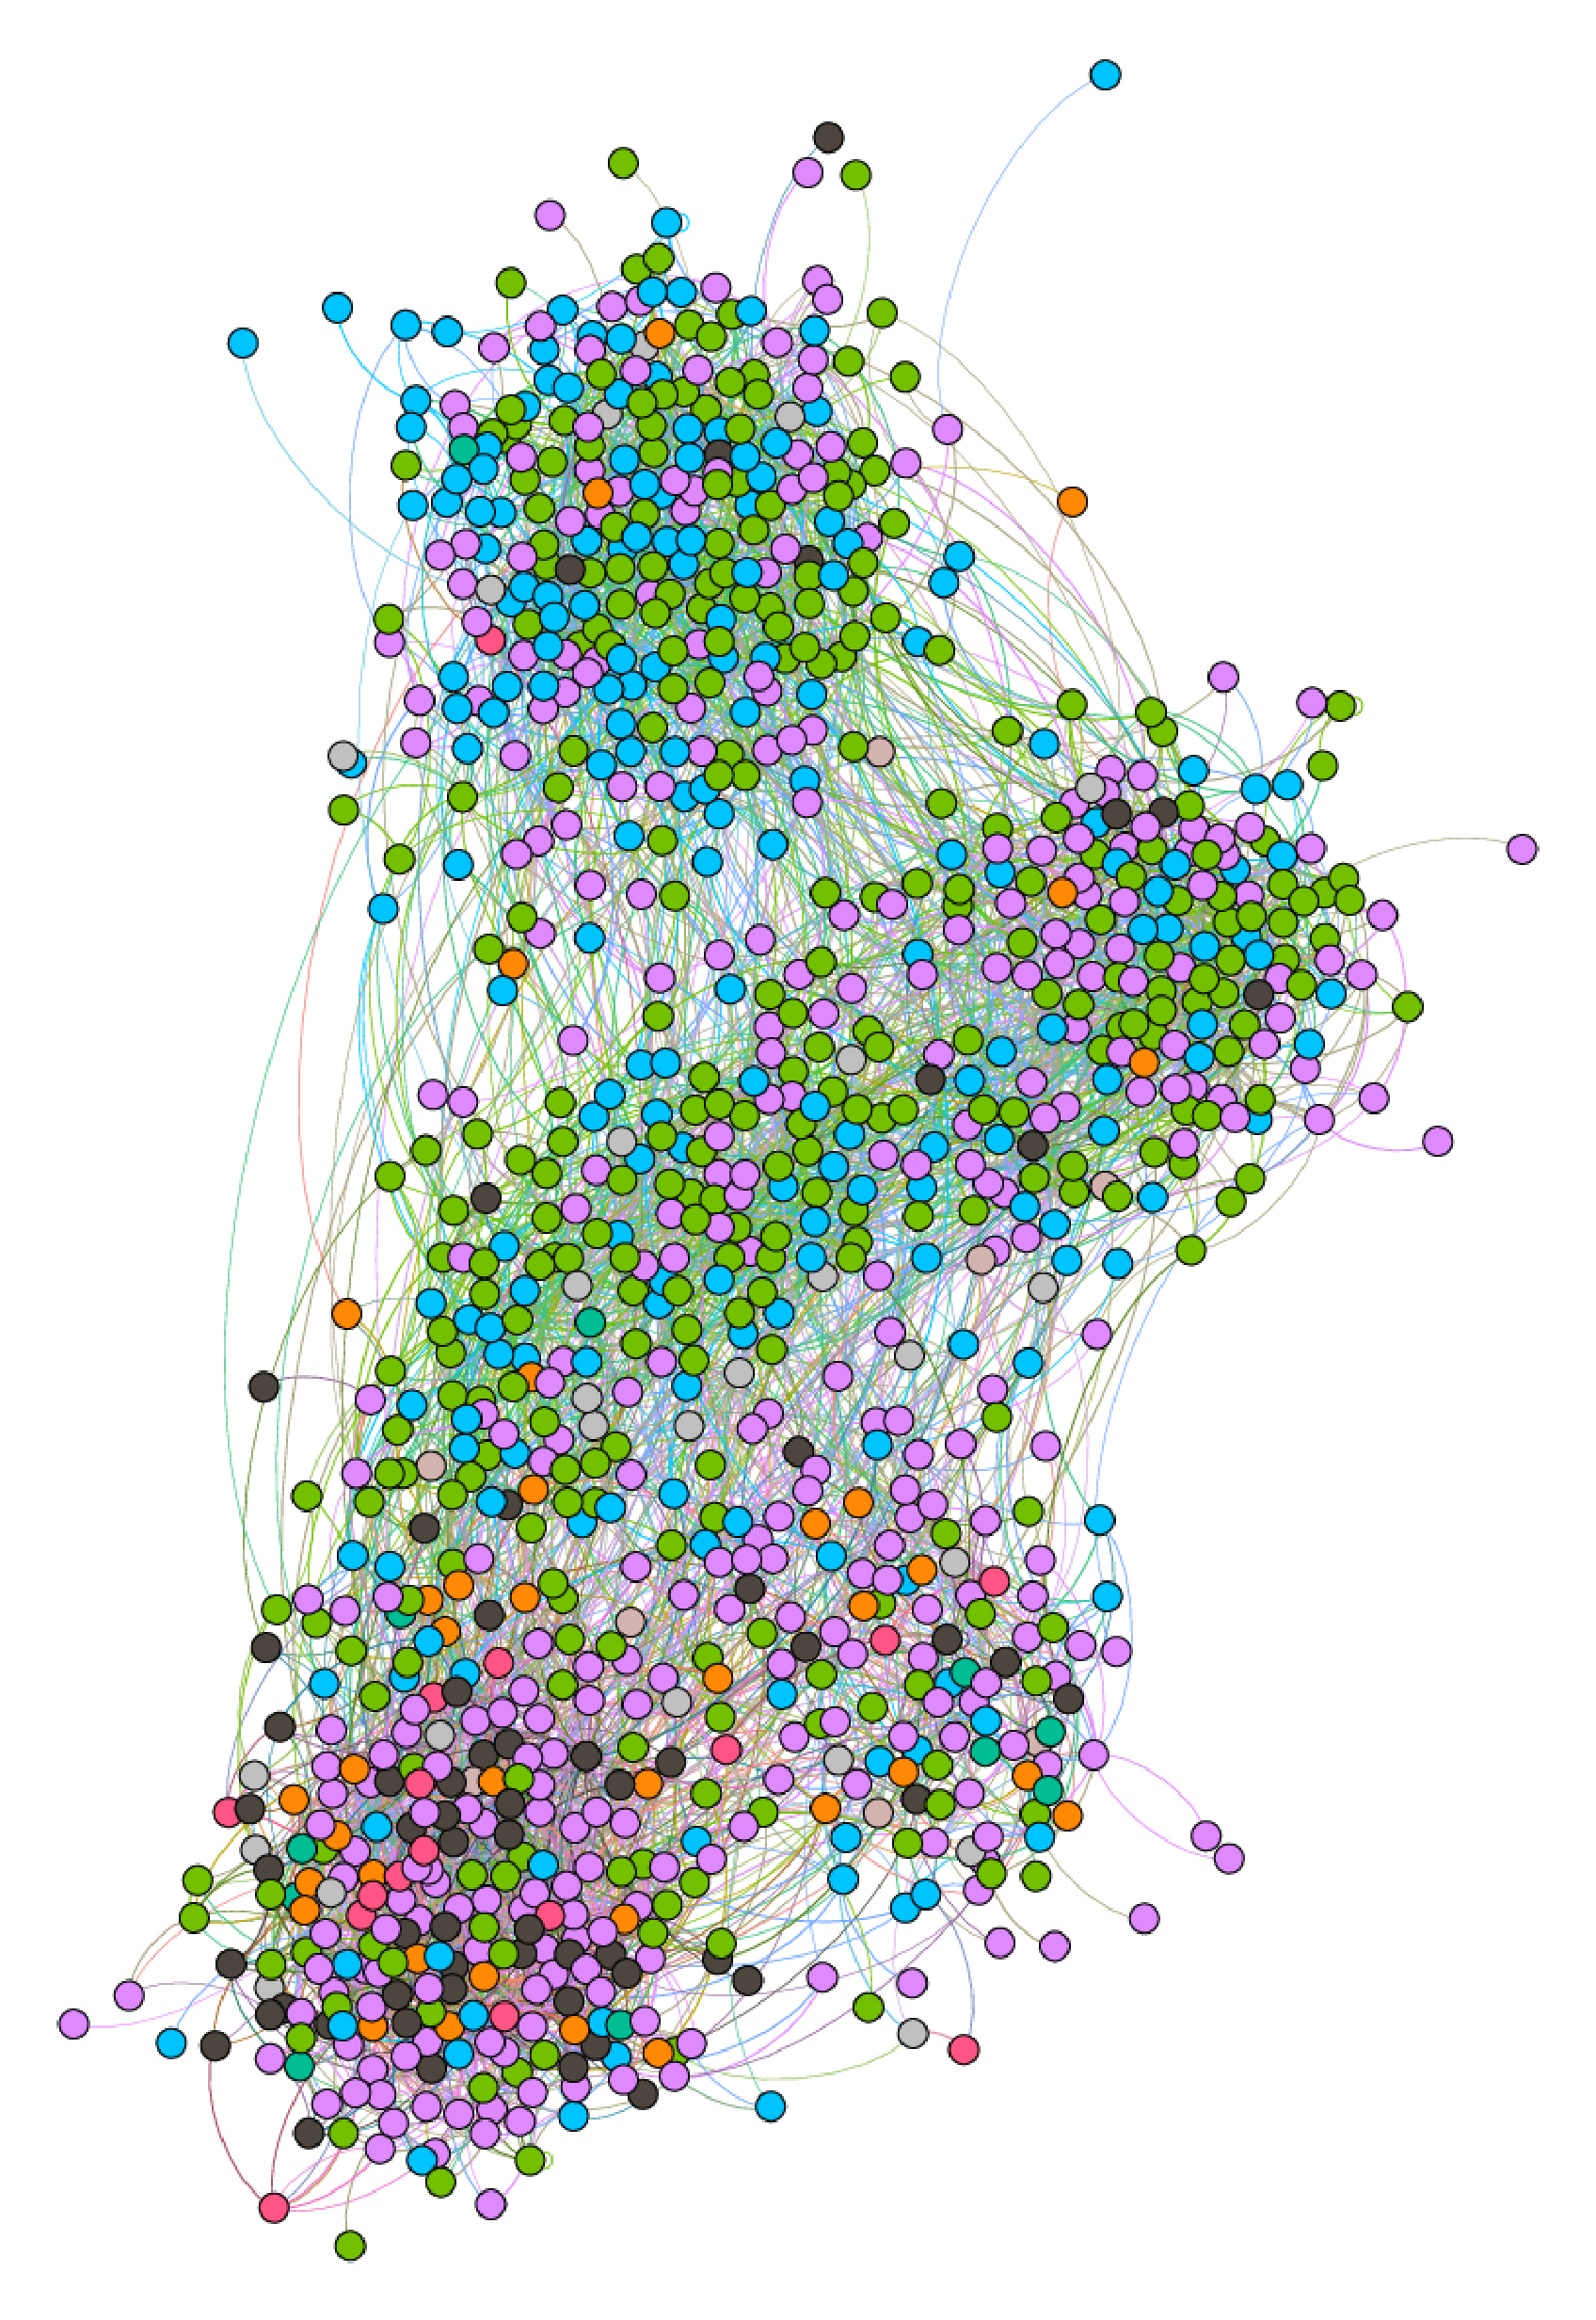
\includegraphics[width=\textwidth]{img/dim5_news.pdf}
    \label{fig:bubble5news}
    \caption{bubble3news}
  \end{subfigure}
  ~
  \begin{subfigure}[t]{0.35\textwidth}
    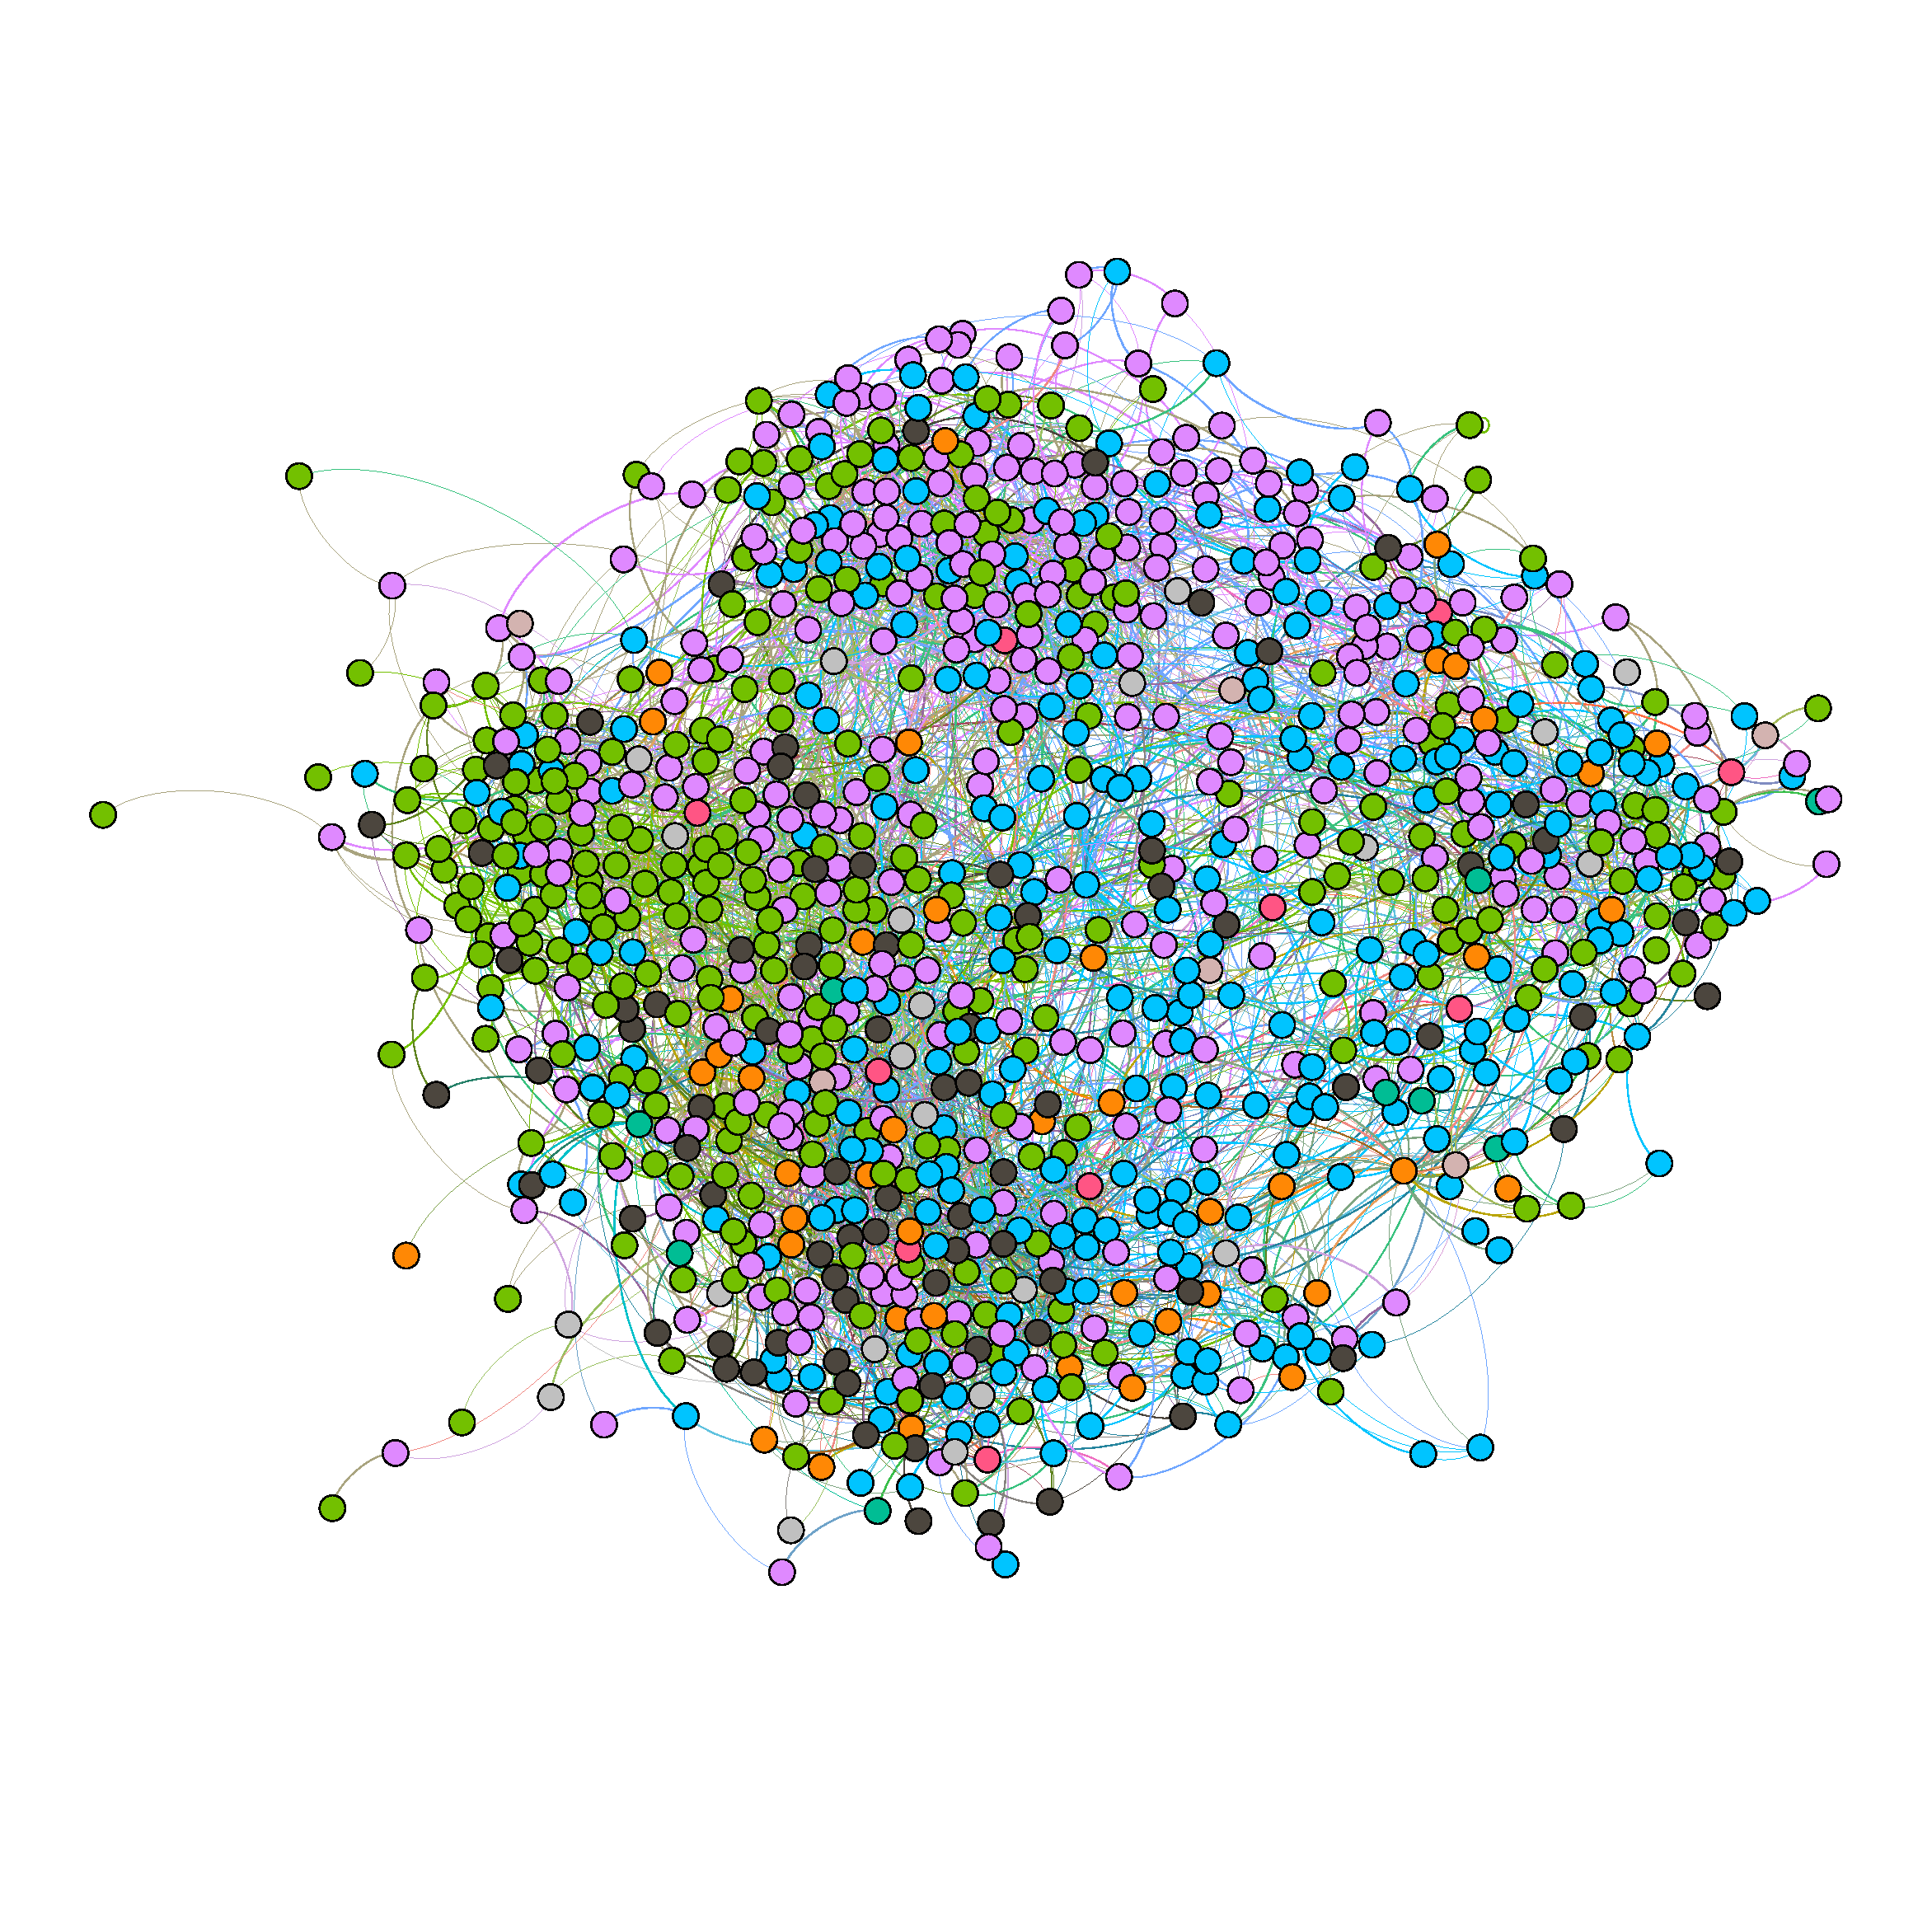
\includegraphics[width=\textwidth]{img/dim7_news.pdf}
    \label{fig:bubble5news}
    \caption{bubble3news}
  \end{subfigure}
  \caption{Simulations for 1000 users and 20 sources after 1000
    iterations. (\ref{fig:bubble3mod}), (\ref{fig:bubble5mod}) and
    (\ref{fig:bubble7mod}) highlights state vector.
    (\ref{fig:bubble3news}), (\ref{fig:bubble3news}) and
    (\ref{fig:bubble3news}) hightlitghts different news.
}
  \label{fig:test}
\end{figure}
